\documentclass[12pt]{article}
\usepackage{graphicx}

\begin{document}

\huge Use Case Details

\begin{itemize}

\item \large Create Employee\\
Figure 1 depicts how an applicant applies to be a broker, and how the Manager is involved in the process.

\begin{figure}[h]
\centering
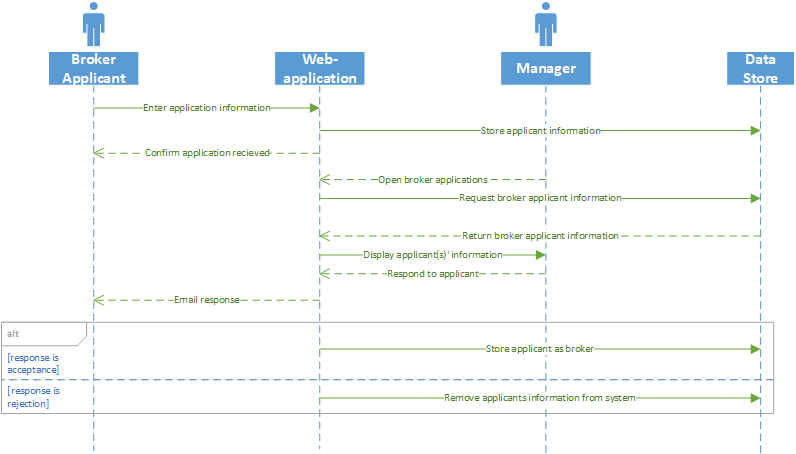
\includegraphics[scale=0.8]{SSDCreateEmployeeV1}
\caption{System Sequence Diagram (SSD) for the 'Create Employee' use case}
\end{figure}


\item \large Create Home Application\\
Figure 2 depicts the steps taken by customer to create a new home application.

\begin{figure}[h]
\centering
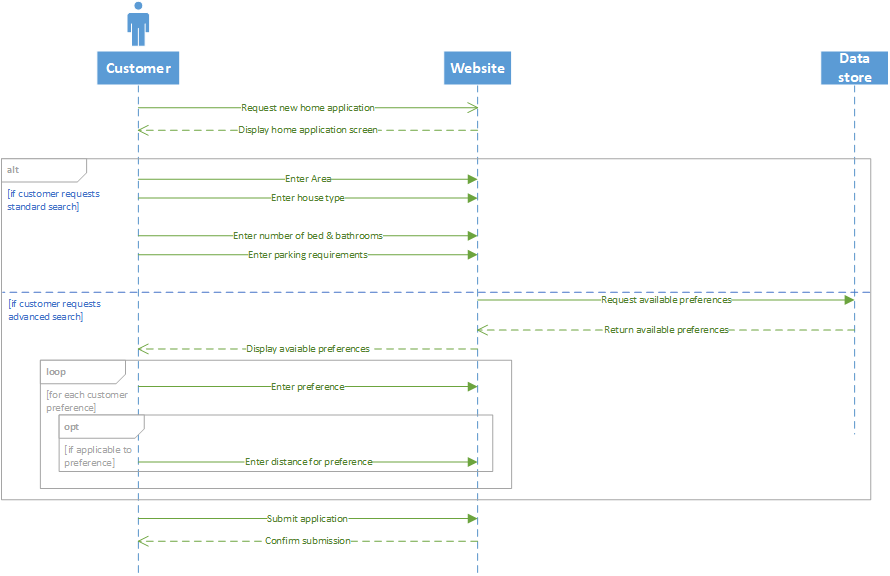
\includegraphics[scale=0.7]{SSDCreateHomeApplication}
\caption{System Sequence Diagram for the 'Create Home Application' use case}
\end{figure}

\item Create Home Suggestion\\
This use case involves the 3 main parts: the system, the application (includes the customer preferences) and the Google Maps API (GMAPI).\\
After the customer has made an application for a smart home selection, the system will request the location of all the customers preferences in the vicinity of the customers preferred area from the GMAPI (for example, if the customer wanted a nearby hospital and to live in Sandton, all the hospitals near Sandton would be retrieved).\\
From there, the System will retrieve all the available homes in the relevant area and will cross reference them with the applications preferences.

\item Home Management\\
This entails the adding and removing of new houses. When a customer has registered themself as a user, they will be able to search for or by a house\\
Selling: To sell a house the customer will select a 'Sell House' option after logging in and enter all the relevant information in (number of rooms, bathrooms, etc.). Thereafter a broker will go to the house and confirm the details.
Buying: After the house has been recorded in the data store, it can be recommended to a buyer. After a buyer has viewed the house and buys it, the house will be marked as sold (it will not be deleted for possible reporting services).
Below is figure 3, that shows the state of the house and what action must be taken to alter the state.

\begin{figure}[h]
\centering
\includegraphics[scale=0.7]{StateMachineDiagramHome}
\caption{State Machine Diagram for the status of a home}
\end{figure}


\item Transaction Management\\
Transactions will be recorded by the manager. The transaction will record the seller, buyer, broker that sold the house and the manager that recorded the sale. If the payment is made through the web application it will be approved by the manager before the sale is confirmed and if the payment is made by other means (such as a cheque)  the manager must manually add the sale for it to be confirmed.

\item Create Home Suggestion\\
Figure 4 is the SSD showing the interaction between the application, the data store and the GMAPI.

\begin{figure}[h]
\centering
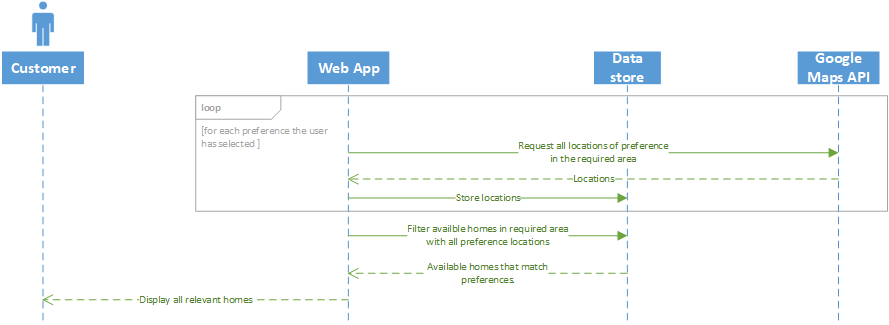
\includegraphics[scale=0.7]{SSDCreateHomeSuggestion}
\caption{System Sequence Diagram for the 'Create Home Suggestion' use case}
\end{figure}
\end{itemize}
\end{document}